\section{Descripción y convenciones del modelo}

La Fig.~\ref{fig:sistema} muestra el esquema adoptado. La coordenada generalizada $y(t)$ describe el desplazamiento vertical de la masa equivalente respecto a su posición de equilibrio estático y se considera positiva hacia arriba. Los extremos superiores del resorte y del amortiguador se conectan a un chasis fijo; sus extremos inferiores actúan sobre el eje asociado a la masa equivalente.

\begin{figure}[t]
  \centering
  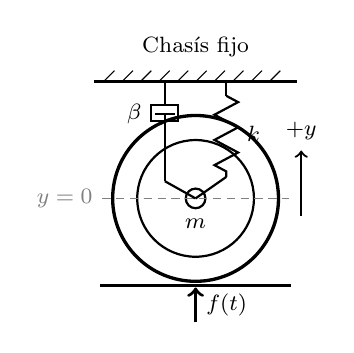
\begin{tikzpicture}[
  scale=0.78,
  every node/.style={font=\footnotesize},
  spring/.style={decorate,decoration={zigzag,segment length=3.2mm,amplitude=1.5mm}}
]
  % Chasís fijo
  \draw[very thick] (-1.65,1.90) -- (1.65,1.90);
  \foreach \x in {-1.5,-1.2,...,1.5}
    \draw[thin] (\x,1.90) -- ++(0.18,0.18);
  \node[anchor=south] at (0,2.15) {Chasís fijo};

  % Rueda y eje
  \draw[very thick] (0,0) circle (1.35);
  \draw[thick] (0,0) circle (0.95);
  \draw[fill=white,thick] (0,0) circle (0.16);
  \node[anchor=north] at (0,-0.18) {$m$};

  % Línea de equilibrio
  \draw[densely dashed,gray] (-1.52,0) -- (1.52,0);
  \node[anchor=east,gray] at (-1.52,0) {$y=0$};

  % Amortiguador
  \draw[thick] (-0.50,1.90) -- (-0.50,1.52);
  \draw[thick] (-0.72,1.26) rectangle (-0.28,1.52);
  \draw[thick] (-0.66,1.38) -- (-0.34,1.38);
  \draw[thick] (-0.50,1.38) -- (-0.50,0.28);
  \draw[thick] (-0.50,0.28) -- (0,0);
  \node[anchor=east] at (-0.72,1.38) {$\beta$};

  % Resorte
  \draw[thick] (0.50,1.90) -- (0.50,1.67);
  \draw[thick,spring] (0.50,1.67) -- (0.50,0.35);
  \draw[thick] (0.50,0.35) -- (0,0);
  \node[anchor=west] at (0.68,1.05) {$k$};

  % Suelo y fuerza
  \draw[very thick] (-1.55,-1.42) -- (1.55,-1.42);
  \draw[->,very thick] (0,-2.02) -- (0,-1.45)
    node[midway,right] {$f(t)$};

  % Coordenada positiva
  \draw[->,thick] (1.72,-0.28) -- (1.72,0.78)
    node[above] {$+y$};
\end{tikzpicture}


  \caption{Modelo simplificado de la rueda con resorte, amortiguador y fuerza perturbadora del terreno.}
  \label{fig:sistema}
\end{figure}

La entrada $f(t)$ no representa la fuerza normal total, sino su variación respecto al valor estático. Si $N(t)$ es la fuerza normal total y $N_0$ su valor de equilibrio, entonces
\begin{equation}
  N(t)=N_0+f(t).
\end{equation}
En el equilibrio, la fuerza normal estática compensa el peso de la masa equivalente y la carga estática transmitida por la suspensión. Por ello, al medir $y(t)$ desde dicha posición, las contribuciones constantes se cancelan y no aparecen en la ecuación dinámica incremental.

\begin{table}[t]
  \caption{Variables y parámetros del modelo}
  \label{tab:simbolos}
  \centering
  \begin{tabular}{@{}cll@{}}
    \toprule
    Símbolo & Descripción & Unidad \\
    \midrule
    $m$ & Masa equivalente de la rueda & \si{\kilogram} \\
    $k$ & Rigidez equivalente del resorte & \si{\newton\per\meter} \\
    $\beta$ & Coeficiente de amortiguamiento & \si{\newton\second\per\meter} \\
    $y(t)$ & Desplazamiento desde el equilibrio & \si{\meter} \\
    $f(t)$ & Fuerza perturbadora del terreno & \si{\newton} \\
    \bottomrule
  \end{tabular}
\end{table}

El desarrollo supone movimiento exclusivamente vertical, parámetros constantes, comportamiento lineal del resorte y amortiguamiento viscoso lineal. También se desprecia la masa propia del resorte y del amortiguador.
